\documentclass{article}
\usepackage{apacite}
\usepackage[T1]{fontenc}
\usepackage{graphicx}
\usepackage{booktabs}
\usepackage{float}
\usepackage{caption}
\usepackage[authoryear]{natbib}
\bibliographystyle{apa}
\usepackage{setspace}
\usepackage{longtable}
\usepackage{array}
\usepackage{geometry}
\usepackage{url}

\title{Practicum Report}
\author{Robert Esposito \\ Rutgers University}
\date{Summer 2024}

\begin{document}

\maketitle

\newpage

\tableofcontents

\newpage

\listoffigures

\newpage

\listoftables

\newpage

\doublespacing

\section{Introduction: Interning at the Manhattan District Attorney's Office's Language Unit}

During Spring 2024, I interned at the Manhattan District Attorney’s Office’s Language Unit as a Spanish interpreter for four months (16 hours per week) in fulfillment of the Spanish Translation and Interpreting Masters’ Program requirements. During my tenure at the office, I developed my skills as a legal interpreter and translator. I learned about the requirements, professional norms and expectations of an interpreter in this professional environment, as compared to other professional interpreting experiences that I have had, such as medical or community interpreting. Through this essay, I will explore the functions of the Language Unit, my responsibilities, what I have learned, the skills I have developed, and the challenges faced.

Approximately 20\% of the 1,694,251 individuals living in Manhattan report that they speak only Spanish at home \citep{us_census_bureau2023}, which indicates the vital need of language services as part of our legal system. Language services are codified into law by Federal, State, and Local laws in New York City as a whole. For example, Title VI of the Civil Rights Act of 1964 requires that courts receiving federal funding must provide access to linguistic services for individuals with limited English proficiency; New York State Judiciary Law § 390 requires linguistic services for individuals with limited English proficiency; and the New York City Administrative Code requires any city agencies to provide interpretation and translation service access to non-English speakers.

New York City is divided into five boroughs, each with their only District Attorney’s Office. The Language Unit at the Manhattan District Attorney’s Office provides language services to the Assistant District Attorneys in various ways for cases in Manhattan. Interpreters will provide language services for office interviews and phone calls with witnesses or victims, judicial proceedings, and occasionally public presentations. Although the job titles typically include “interpreter”, and that is how they refer to themselves as, they oftentimes also provide transcription and translation services for phone calls (e.g. from a prison or jail), text messages, police bodycam footage, and 911 calls.

Typically, an interpreter will be assigned in advance to a certain number of interpreting cases in a day, and there will be one interpreter who is “on call” to take phone calls or last-minute interpreting requests. When interpreters are not on a case, they are typically responsible for transcribing and translating the audios, videos, or texts described above.

\section{Interpreting Experiences, Challenges and Lessons Learned}

During my tenure, I assisted in interpretation for office interview and phone calls, as well as transcription and translation services. Through these experiences, I have learned worked to further solidify my understanding of what it means to be an interpreter in the judicial environment. Below, I will highlight some of my experiences and what I gained from them.

\subsection{Language Variation}

The Manhattan District Attorney’s Office serves over 330,000 individuals who only speak Spanish at home, not including individuals who speak English at any proficiency level, but would prefer to navigate in the legal system through Spanish. The Spanish-speaking population are made up of over 20 different ethnic groups, such as Dominican, Honduran, and Mexican \citep{nyc_immigrant_fact_sheet}, each speaking their own variety of Spanish. Although mutually intelligible, each variety of Spanish is modulated by cultural, social, and contextual factors that impact all parts of the language, such as the vocabulary, grammar, and phonology \citep{moreno2019variedades}. At the Manhattan District Attorney’s Office, I encountered this variation first-hand and had to learn how to cope with the grand linguistic diversity within Spanish.

The first interpretation service that I provided was for a phone interview between an Assistant District Attorney and her witness, “María”. When assigned a case, an interpreter is provided with a case file online that includes a police report and some general information about the perpetrator. Unfortunately, for last-minute cases, the interpreter typically does not have time to review the case information. 

Before this case, I had never done telephonic interpretation, and it was a challenging first assignment. It is common for first-time interpreters to be stressed during their initial assignments, which can lead to reduced performance, such as short-term memory failure, due to anxieties \citep{yang_tan2017}. 
Another challenge for this assignment was the variety of Spanish that María spoke, Dominican Spanish. Despite Dominicans making up the largest percentage of Latinx immigrants in New York City at about 41\% \citep{nyc_immigrant_fact_sheet}, I do not have much experience interacting with Dominicans or hearing their language use. For example, María used the word truncar when talking about her travel plans being thwarted, a word that I did not recognize. Her phonological patterns also made it difficult for me to parse her speech, requiring me to use more cognitive effort than I would have to for other varieties of Spanish, taking away from cognitive resources that should have been devoted to working memory.

These two issues are within my control, and I became aware of the need to familiarize myself better with the population that the District Attorney’s Office serves, as well as work on coping mechanisms to prevent short-term memory failure. My advisor suggested that I utilize social media, such as Instagram, to find Dominican influencers (or any other variety as needed) who speak explicitly about the linguistic diversity within the Dominican Republic. Other methods include watching Dominican media or listening to Dominican music.

\subsection{Fulfilling Interpreting Ethics}

Later in my tenure, I provided interpreting services for a witness, “Carla”, in an office interview with an Assistant District Attorney. With my first-time nerves out of the way, and having shadowed other interpreters for office interviews, I felt more comfortable, but I still felt anxiety that my advisor was listening in on the interpretation and that it was official business. 

My short-term memory did not fail as often, and she was Venezuelan, a variety of Spanish with which I am more familiar through other interpreting jobs. However, the cognitive tools at my disposal to work around linguistic issues and my theoretical knowledge of best practices sometimes did not surface as quickly as they should have, possibly due to anxiety. For example, the Assistant District Attorney asked, “Did he smash it, break it, snap it?” The semantically similar words made me stumble, and I unfortunately was not able to provide a full and accurate interpretation. I was able to provide the correct words for smash and break, but for snap, I had to resort to a hand gesture.

Although the message was communicated for the purpose of the interview, my actions did not align with standard interpreter ethics. The \citet{najit_code_of_ethics} specifies that “[s]ource-language speech should be faithfully rendered into the target language” , which I was unable to do at that time. Although I was aware of the ethical requirements of me as an interpreter, it is important to internalize these practices so that at the time of interpretation, they can be automatized under pressure.

\subsection{Managing the Flow of Conversation}

Within interpreting studies, there is an on-going debate about the interpreter’s (in)visibility. Although it is commonly taught, such as within my own experience during Masters’ program, that interpreters are meant to be “invisible” and only work as the voices of the interlocutors, there are various ways that an interpreter “becomes visible”. One such way is through setting communication rules at the beginning of or during the encounter, as well as controlling the traffic of information \citep{roy2000interpreting}. For example, an interpreter may explicitly set the rule that if they raise their hand, the interlocutors should pause speaking to give the interpreter a chance to interpret the utterance. The interpreter may choose to pause the interlocutor due to a strain on their working memory.

In another case, I had to grapple with “becoming visible” and managing the flow of conversation. I interpreted for “Ana” in an office interview with an Assistant District Attorney. In this case, I learned about managing the interlocutors and being more flexible. In the beginning, the client was partially covering her mouth and speaking softly, making it difficult to hear her utterances. My advisor noticed this, and she communicated the issue to the Assistant District Attorney, with the best practice of speaking in the third person, and the issue was resolved when he asked the client to move her hand away from her mouth and to speak louder. This demonstrated to me a situation in which it is necessary to “become visible” as the interpreter, and the best practices of doing so. That is, communicating in the third person to the service provider, not to the LEP.

Office interviews are typically conducted in the simultaneous mode to expedite the encounter, as was this one. However, the witness had to call someone. At this point, my advisor indicated for me to switch to consecutive, due to the poor quality of the phone call. Given the chaotic environment that interpreters can find themselves in, it is necessary to be flexible about their services. However, to provide the accurate service as required by NAJIT, an interpreter must “become visible” and advocate for their needs. A consistent issue that I had throughout my interpreting experiences was difficulty in managing the length of utterances in consecutive interpretation. Although I theoretically know how much information I can receive before straining my working memory, something I have demonstrated this to myself at other interpreting jobs outside of the Manhattan District Attorney’s Office, I found it difficult to intervene when an Assistant District Attorney or LEP began to speak for too long. In this instance, I found it difficult to “become difficult” to interrupt the LEP. Since I have been able to intervene in other instances, I think that the source of my difficulties lies in the environment: I may have been intimidated by the authority position of the Assistant District Attorney, as well as anxious about having my advisor listening to my interpretation. 

As it is common for interpreters to have to interact with people in positions of authority, as well as to be observed by supervisors for quality control, this is an issue that I must control internally. For example, I need to desensitize myself to these factors, as well as create an automaticity of the action. The latter can be done through having a “script” already prepared of what to say when I need to intervene in English or Spanish.

\subsection{Notetaking}

Another mechanism that should be used in tandem with controlling the flow of conversation is notetaking. While completing my internship, I was also taking a medical interpreting course, where we explicitly worked on notetaking skills. Although the contexts are different, thus generally focusing on a different set of semantic vocabulary, the notetaking skills I was acquiring in that course helped me to begin developing my own notetaking practices and symbols that could be applied more generally. 

Due to the great variety of cases, it was difficult to quickly come up with shorthand symbols that would benefit me during the interpreting encounter. However, when I was able to see the case report before interpreting, I would imagine key words that might come up. For example, for a domestic violence case, I made or reviewed symbols for spouse, child, house/home, hospital, hit. When vocabulary did come up, the symbols helped to put less strain on my working memory. The greatest benefit I found for notetaking was with sequence of events, and I hope to continue developing my notetaking skills to assist me with this. When an interlocutor is recounting a story, either to explain what happened (e.g. the witness or victim) or to verify information (e.g. the Assistant District Attorney), I found that notetaking helped to less the cognitive load of the sequence.

Interestingly, I found that the majority of the interpreters did not utilize notetaking for their encounters. If they did bring a notebook with them, they usually utilized it very infrequently. Only one interpreter consistently took notes throughout her interpretations. For other interpreters, I found that they mainly used notetaking to write down proper names (e.g. names of people, addresses) or numbers, which I was taught during my coursework are some of the most important things to take notes of. Another time that they frequently used notetaking was when they encountered a difficult item for interpretation, which they would bring back to the Language Unit to discuss with their colleagues about possible translation solutions.

During my interpretation encounters, I was made aware of the necessity to hone my notetaking skills. Although it is not something actively used by all interpreters, it is yet another resource that can be taken advantage of to lessen the cognitive load of the encounter. 

\subsection{Transcription and Translation Services}

Outside of interpreting services, I also provided transcription and translation services. During my time at the office, I transcribed and translated 911 calls, police interviews, and police bodycam footage. This gave me a greater opportunity to get exposure to the populations that the office serves. Although I was already familiar with transcription and translation practices from a theoretical perspective through classwork, having specific professional standards and best practices to abide by gave me a new perspective. I was glad to see that what I learned in class held up to the professional environment, with minor tweaks that were specific to the environment. For example, specific formatting that is required by the office, as well as greater familiarity with affidavits of translation.

\section{Timetables}

As previously described, I performed a variety of tasks while interning at the Manhattan District Attorney’s Office. I categorized these tasks into 8 categories, the criteria of which are displayed in Table 1. These categories include Human Resources (HR), independent study, preparation, shadow, interpretation, guided review, translation, and transcription. It should be noted that all transcription tasks involved translating the transcribed audios, as well.

\begin{table}[H]
\centering
\caption{Task types and criteria for the category.} 
\label{tab:task_types}
\begin{tabular}{lp{10cm} lp{5cm}}
\toprule
Task type & Definition\\
\midrule
\addlinespace
HR & Tasks assigned by HR, such as obligatory Title IX training videos.\\
\addlinespace
Independent study & Tasks explicitly or not explicitly assigned to me, such as studying legal vocabulary or reading scholarly articles on legal translation.\\
\addlinespace
Preparation & Tasks that prepared me for shadowing or interpreting assignments.\\
\addlinespace
Shadow & Shadowing interpreters.\\
\addlinespace
Interpretation & Interpretation and screening of videos or audios.\\
\addlinespace
Guided review & Review with one of the interpreters of an interpretation or translation.\\
\addlinespace
Translation & Translation of a document.\\
\addlinespace
Transcription & Transcription and translation of a video or audio.\\
\addlinespace
Glossary & Work on creating and maintaining a glossary.\\
\bottomrule
\end{tabular}
\end{table}

Table 2 lays out the tasks that I did at the Manhattan District Attorney’s Office. It includes the date of the task, at what time I began the task, at what time I ended the task, the task itself, and the type of task.

\begin{longtable}{lp{1.8cm} l p{5cm} l p{1.5cm} l p{5cm} l p{5cm}}
\caption{Timetables for my internship at the Manhattan DA's Office. The table includes the date, the time starting and ending a task, the task, and the type of task.} \label{tab:tasks} \\
\toprule
Date & Start time & End time & Task & Type\\
\midrule
\endfirsthead

\multicolumn{5}{c}%
{Table \thetable: Continued from previous page} \\
\toprule
Date & Start time & End time & Task & Type\\
\midrule
\endhead

\midrule
\multicolumn{5}{r}{\textit{Continued on next page}} \\
\endfoot

\bottomrule
\endlastfoot

2/14/2024 & 09:30 & 11:00 & IT training & HR\\
2/14/2024 & 11:00 & 13:00 & Review introductory material from District Attorney's Office & independent study\\
2/14/2024 & 02:00 & 16:30 & Review introductory material from District Attorney's Office & independent study\\
2/16/2024 & 09:00 & 10:00 & timekeeping training & HR\\
2/16/2024 & 10:00 & 13:00 & Review introductory material from District Attorney's Office & independent study\\
\addlinespace
2/16/2024 & 14:00 & 14:30 & Orientation & independent study\\
2/16/2024 & 14:30 & 16:30 & Review bodycam footage & preparation\\
2/20/2024 & 09:30 & 10:30 & Shadow office interview & shadow\\
2/20/2024 & 10:30 & 11:00 & Office interview review with interpreter & guided review\\
2/20/2024 & 11:00 & 13:00 & Study Acebo material & independent study\\
\addlinespace
2/20/2024 & 14:00 & 14:15 & HR training video & HR\\
2/20/2024 & 14:15 & 14:30 & Office interview review with interpreter & guided review\\
2/20/2024 & 14:30 & 16:00 & HR training video & HR\\
2/20/2024 & 16:00 & 16:30 & Review victim impact statements & independent study\\
2/22/2024 & 09:30 & 10:30 & preparation for video screening & preparation\\
\addlinespace
2/22/2024 & 10:30 & 11:00 & domestic incident report translation & translation\\
2/22/2024 & 11:00 & 13:00 & Read Breaking Silence Training Manual & independent study\\
2/22/2024 & 14:00 & 15:00 & HR training video & HR\\
2/22/2024 & 15:00 & 15:10 & video screening for ADA & interpretation\\
2/22/2024 & 15:10 & 16:30 & HR training video & HR\\
\addlinespace
2/27/2024 & 09:30 & 10:30 & HR training video & HR\\
2/27/2024 & 10:30 & 11:00 & interpretation preparation & preparation\\
2/27/2024 & 11:00 & 12:00 & vocabulary review (clothing, physical description) & independent study\\
2/27/2024 & 12:00 & 13:00 & Study Acebo material & independent study\\
2/27/2024 & 14:00 & 16:00 & Study Acebo material & independent study\\
\addlinespace
2/29/2024 & 09:30 & 09:45 & Factual Basis translation & translation\\
2/29/2024 & 09:45 & 10:15 & Read on proffer agreements & preparation\\
2/29/2024 & 10:15 & 10:45 & HR training video & HR\\
2/29/2024 & 10:45 & 11:15 & Review bodycam footage & preparation\\
2/29/2024 & 11:15 & 11:30 & HR training video & HR\\
\addlinespace
2/29/2024 & 11:30 & 12:00 & Review proffer agreement and translation & preparation\\
2/29/2024 & 13:00 & 14:00 & shadow Proffer interview & shadow\\
2/29/2024 & 14:00 & 14:30 & Proffer review with interpreter & guided review\\
2/29/2024 & 14:30 & 15:00 & Proffer review & independent study\\
2/29/2024 & 15:00 & 16:00 & shadow office interview & shadow\\
\addlinespace
2/29/2024 & 16:00 & 16:30 & Office interview review with interpreter & guided review\\
3/5/2024 & 09:30 & 10:30 & HR training video & HR\\
3/5/2024 & 10:30 & 11:00 & HR training video & HR\\
3/5/2024 & 11:00 & 11:30 & glossary creation & glossary\\
3/5/2024 & 11:30 & 13:00 & 911 call transcription and translation & transcription\\
\addlinespace
3/5/2024 & 14:00 & 16:00 & shadow proffer session & shadow\\
3/5/2024 & 16:00 & 16:30 & 911 call transcription and translation & transcription\\
3/7/2024 & 09:30 & 11:00 & Review details and vocab for cases & preparation\\
3/7/2024 & 11:00 & 12:00 & 911 call transcription and translation & transcription\\
3/7/2024 & 12:00 & 12:30 & Read articles on legal translation & independent study\\
\addlinespace
3/7/2024 & 12:30 & 13:00 & 911 call transcription and translation & transcription\\
3/7/2024 & 14:00 & 14:15 & Read articles on legal translation & independent study\\
3/7/2024 & 14:15 & 15:00 & Review Rikers call & preparation\\
3/7/2024 & 15:00 & 15:30 & telephonic interpretation & interpretation\\
3/7/2024 & 15:30 & 16:00 & 911 call transcription and translation & transcription\\
\addlinespace
3/7/2024 & 16:00 & 16:30 & Read articles on legal translation & independent study\\
3/12/2024 & 09:30 & 10:45 & Read articles on legal translation & independent study\\
3/12/2024 & 10:45 & 11:15 & translate domestic incident report & translation\\
3/12/2024 & 11:15 & 13:00 & Shadow office interview & shadow\\
3/12/2024 & 14:00 & 14:15 & Read legal translation article & independent study\\
\addlinespace
3/12/2024 & 14:15 & 15:00 & shadow Proffer interview & shadow\\
3/12/2024 & 15:00 & 15:30 & review translation with interpreter & guided review\\
3/12/2024 & 15:30 & 16:30 & 911 call transcription and translation & transcription\\
3/14/2024 & 09:30 & 11:15 & Read articles on legal translation & independent study\\
3/14/2024 & 11:15 & 12:00 & translate three domestic incident reports & translation\\
\addlinespace
3/14/2024 & 12:00 & 12:30 & Read articles on legal translation & independent study\\
3/14/2024 & 12:30 & 13:00 & translate three domestic incident reports & translation\\
3/14/2024 & 14:30 & 16:00 & Review 911 transcription/translation, domestic incident reports, and misdemeanor factual basis & guided review\\
3/14/2024 & 16:00 & 16:30 & Edit domestic incident reports & translation\\
3/19/2024 & 09:30 & 10:00 & HR training video & HR\\
\addlinespace
3/19/2024 & 10:00 & 11:00 & Read articles on legal translation & independent study\\
3/19/2024 & 11:00 & 11:15 & Update internal units glossary & glossary\\
3/19/2024 & 11:15 & 11:45 & Read articles on legal translation & independent study\\
3/19/2024 & 11:45 & 12:45 & shadow office interview & shadow\\
3/19/2024 & 12:45 & 13:00 & Read articles on legal translation & independent study\\
\addlinespace
3/19/2024 & 14:00 & 15:00 & Read articles on legal translation & independent study\\
3/19/2024 & 15:30 & 16:00 & shadow office interview & shadow\\
3/19/2024 & 16:00 & 16:30 & Read articles on legal translation & independent study\\
3/21/2024 & 09:30 & 09:45 & Update internal units glossary & glossary\\
3/21/2024 & 09:45 & 10:00 & Read articles on legal translation & independent study\\
\addlinespace
3/21/2024 & 10:00 & 10:15 & review upcoming cases & preparation\\
3/21/2024 & 10:15 & 11:00 & Review strangulation domestic violence presentation & preparation\\
3/21/2024 & 11:00 & 11:45 & Read articles on legal translation & independent study\\
3/21/2024 & 11:45 & 12:15 & Transcribe/translate NYPD interview & transcription\\
3/21/2024 & 12:15 & 12:45 & telephonic interpretation & interpretation\\
\addlinespace
3/21/2024 & 12:45 & 13:00 & Transcribe/translate NYPD interview & transcription\\
3/21/2024 & 14:00 & 16:30 & Transcribe/translate NYPD interview & transcription\\
3/24/2024 & 09:30 & 10:30 & domestic incident report translation & translation\\
3/24/2024 & 10:30 & 11:30 & Read medical interpreting ethics & independent study\\
3/24/2024 & 11:30 & 13:00 & shadow proffer & shadow\\
\addlinespace
3/24/2024 & 14:00 & 15:00 & Read medical interpreting ethics & independent study\\
3/24/2024 & 15:00 & 15:30 & Review proffer vocab & guided review\\
3/24/2024 & 15:30 & 16:30 & Read medical terminology chapter & independent study\\
4/2/2024 & 09:30 & 10:30 & Study interpreting ethics & independent study\\
4/2/2024 & 10:30 & 10:45 & Review texts to prepare for screening & preparation\\
\addlinespace
4/2/2024 & 10:45 & 12:30 & shadow office interview & shadow\\
4/2/2024 & 12:30 & 13:00 & Review legal vocab from office interview with interpreter & guided review\\
4/2/2024 & 14:00 & 14:30 & domestic incident report translation & translation\\
4/2/2024 & 14:30 & 16:30 & Study legal terminology & independent study\\
4/4/2024 & 09:30 & 10:30 & Review case information & preparation\\
\addlinespace
4/4/2024 & 10:30 & 12:30 & shadow chuchotage in court & shadow\\
4/4/2024 & 12:30 & 13:00 & screen video & interpretation\\
4/4/2024 & 14:00 & 14:30 & Read articles on legal translation & independent study\\
4/4/2024 & 14:30 & 15:30 & interpret office interview & interpretation\\
4/4/2024 & 15:30 & 16:30 & review office interview interpretation with interpreter & guided review\\
\addlinespace
4/9/2024 & 09:30 & 10:00 & Read articles on legal translation & independent study\\
4/9/2024 & 10:00 & 11:30 & Transcribe/translate NYPD interview & transcription\\
4/9/2024 & 11:30 & 12:00 & review rikers call & preparation\\
4/9/2024 & 12:00 & 13:00 & review vocabulary for current cases & preparation\\
4/9/2024 & 14:00 & 15:00 & translate text messages & translation\\
\addlinespace
4/9/2024 & 15:00 & 15:15 & Read articles on legal translation & independent study\\
4/9/2024 & 15:15 & 15:30 & translate text messages & translation\\
4/9/2024 & 15:30 & 16:30 & Read articles on legal translation & independent study\\
4/12/2024 & 09:30 & 13:00 & Study current cases & preparation\\
4/12/2024 & 14:00 & 16:30 & Study vocabulary & independent study\\
\addlinespace
4/16/2024 & 09:30 & 10:30 & Study current cases & preparation\\
4/16/2024 & 10:30 & 13:00 & Study current cases & preparation\\
4/16/2024 & 14:00 & 15:00 & read psych eval articles & independent study\\
4/16/2024 & 15:00 & 16:30 & Review Rikers call & preparation\\
4/18/2024 & 09:30 & 11:10 & Review cases for the day & preparation\\
\addlinespace
4/18/2024 & 11:10 & 12:30 & screen bodycam footage & interpretation\\
4/18/2024 & 12:30 & 13:00 & translate text messages & translation\\
4/18/2024 & 14:00 & 16:30 & translate text messages & translation\\
4/23/2024 & 09:30 & 10:30 & review bodycam footage for screening & preparation\\
4/23/2024 & 10:30 & 12:00 & Review psych eval footage & independent study\\
\addlinespace
4/23/2024 & 12:00 & 12:20 & bodycam footage screening & interpretation\\
4/23/2024 & 12:20 & 13:00 & Review psych eval footage & independent study\\
4/23/2024 & 14:00 & 16:30 & translate text messages & translation\\
4/25/2024 & 09:30 & 12:30 & translate text messages & translation\\
4/25/2024 & 12:30 & 13:00 & interpret office interview & interpretation\\
\addlinespace
4/25/2024 & 14:00 & 15:30 & federal court shadow & shadow\\
4/25/2024 & 15:30 & 16:30 & translate text messages & translation\\
4/30/2024 & 09:30 & 13:00 & translate antecedentes & translation\\
4/30/2024 & 14:00 & 15:00 & translate antecedentes & translation\\
4/30/2024 & 15:00 & 15:30 & Exit interview & HR\\
\addlinespace
4/30/2024 & 15:30 & 16:30 & translate antecedentes & translation\\
5/2/2024 & 09:30 & 10:00 & review bodycam footage & independent study\\
5/2/2024 & 10:00 & 13:00 & translate criminal complaint document & translation\\
5/2/2024 & 14:00 & 15:00 & Prepare/Redact documents for practicum & translation\\
5/2/2024 & 15:00 & 16:30 & translate criminal complaint document & translation\\
\bottomrule
\end{longtable}

Figure 1 displays raw time in minutes that I spent performing each task. Figure 2 displays the same information as a percentage of my total time. Approximately a third of my time spent at the internship was spent doing independent study, which includes studying material explicitly given to me by my advisors, as well as material outside of the internship that I believed would benefit me, such as scholarly articles on legal translation or interpretation ethics.

Only 3.1\% (280 minutes) of my time was spent interpreting, which includes screening videos and audios for Assistant District Attorneys. This low percentage can be attributed to the high-stakes nature of the field, which at many times requires an interpreter with court interpreting credentials to interpret to prevent any legal issues. Furthermore, some of the tasks were considered too sensitive for me to participate in. For example, there were times at which a female interpreter was requested, which would prevent me from taking the assignment or shadowing.
	
Although transcription and translation are separate categories, note that for all transcription tasks, it was also necessary to translate the transcribed audios. 

\begin{figure}[H]
	\centering
	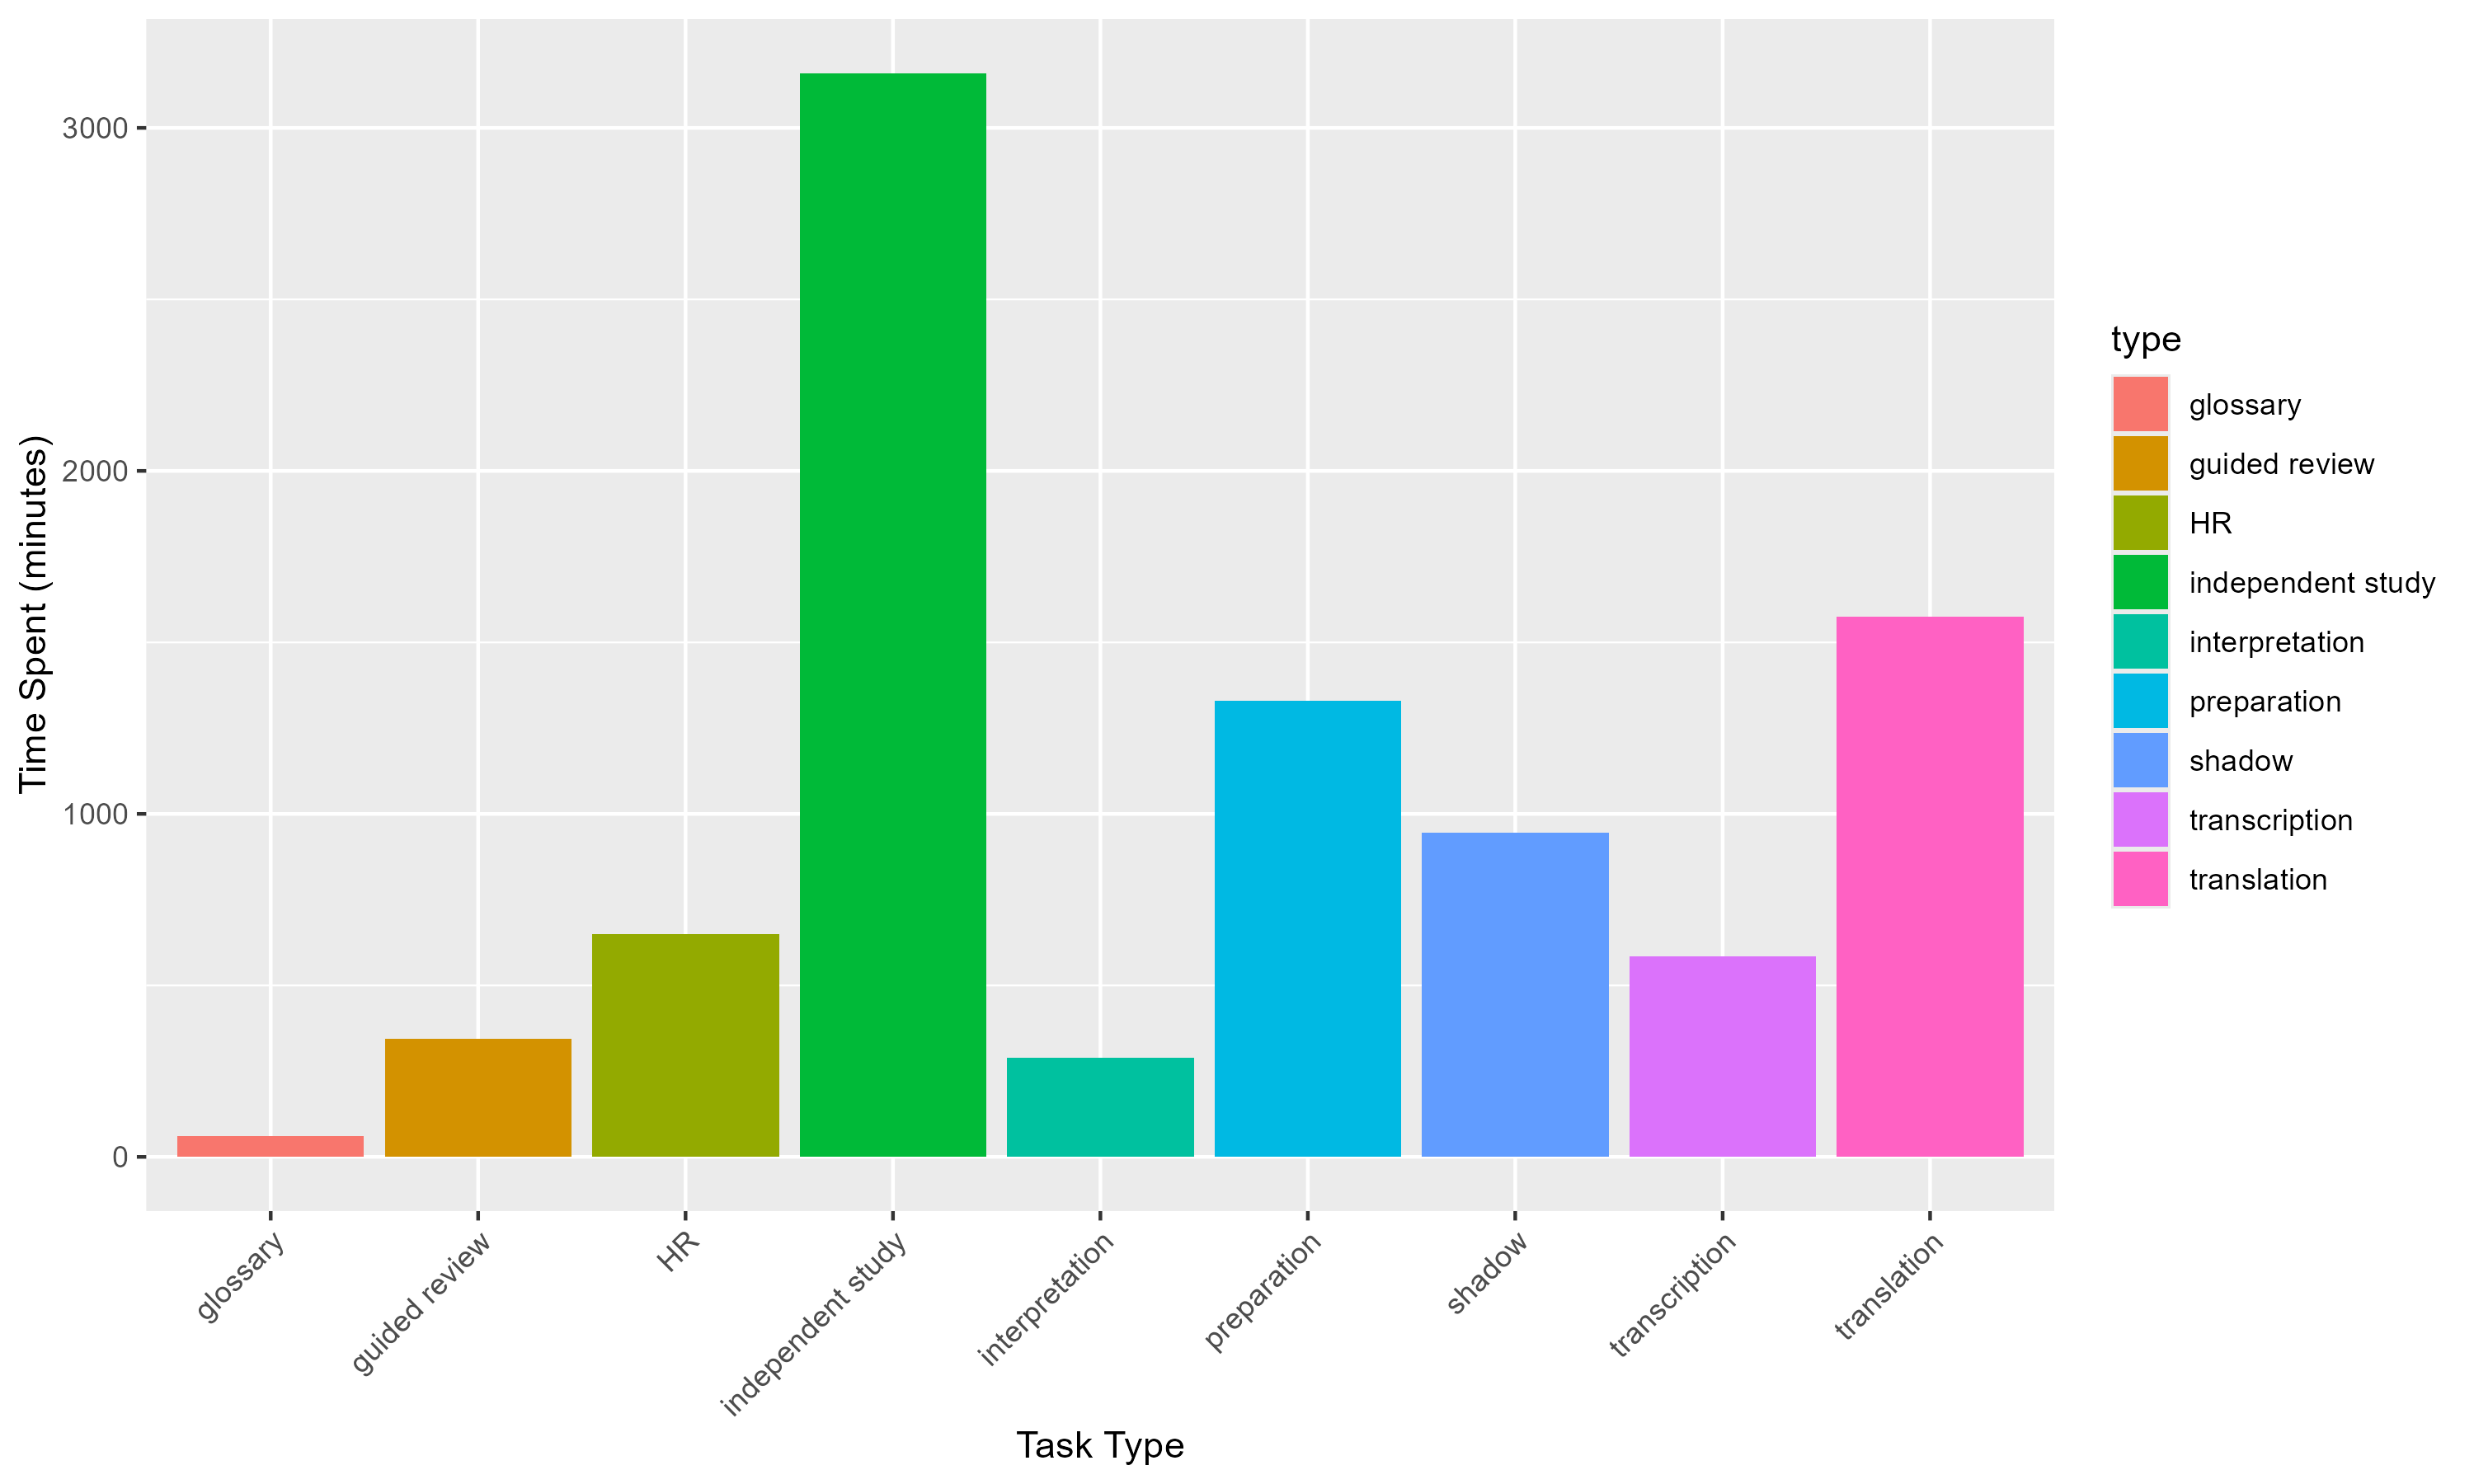
\includegraphics[width=\textwidth]{../figures/bar.png}
	\caption{Total time spent on each task in minutes.}
	\label{fig:bar}
\end{figure}

\begin{figure}[H]
	\centering
	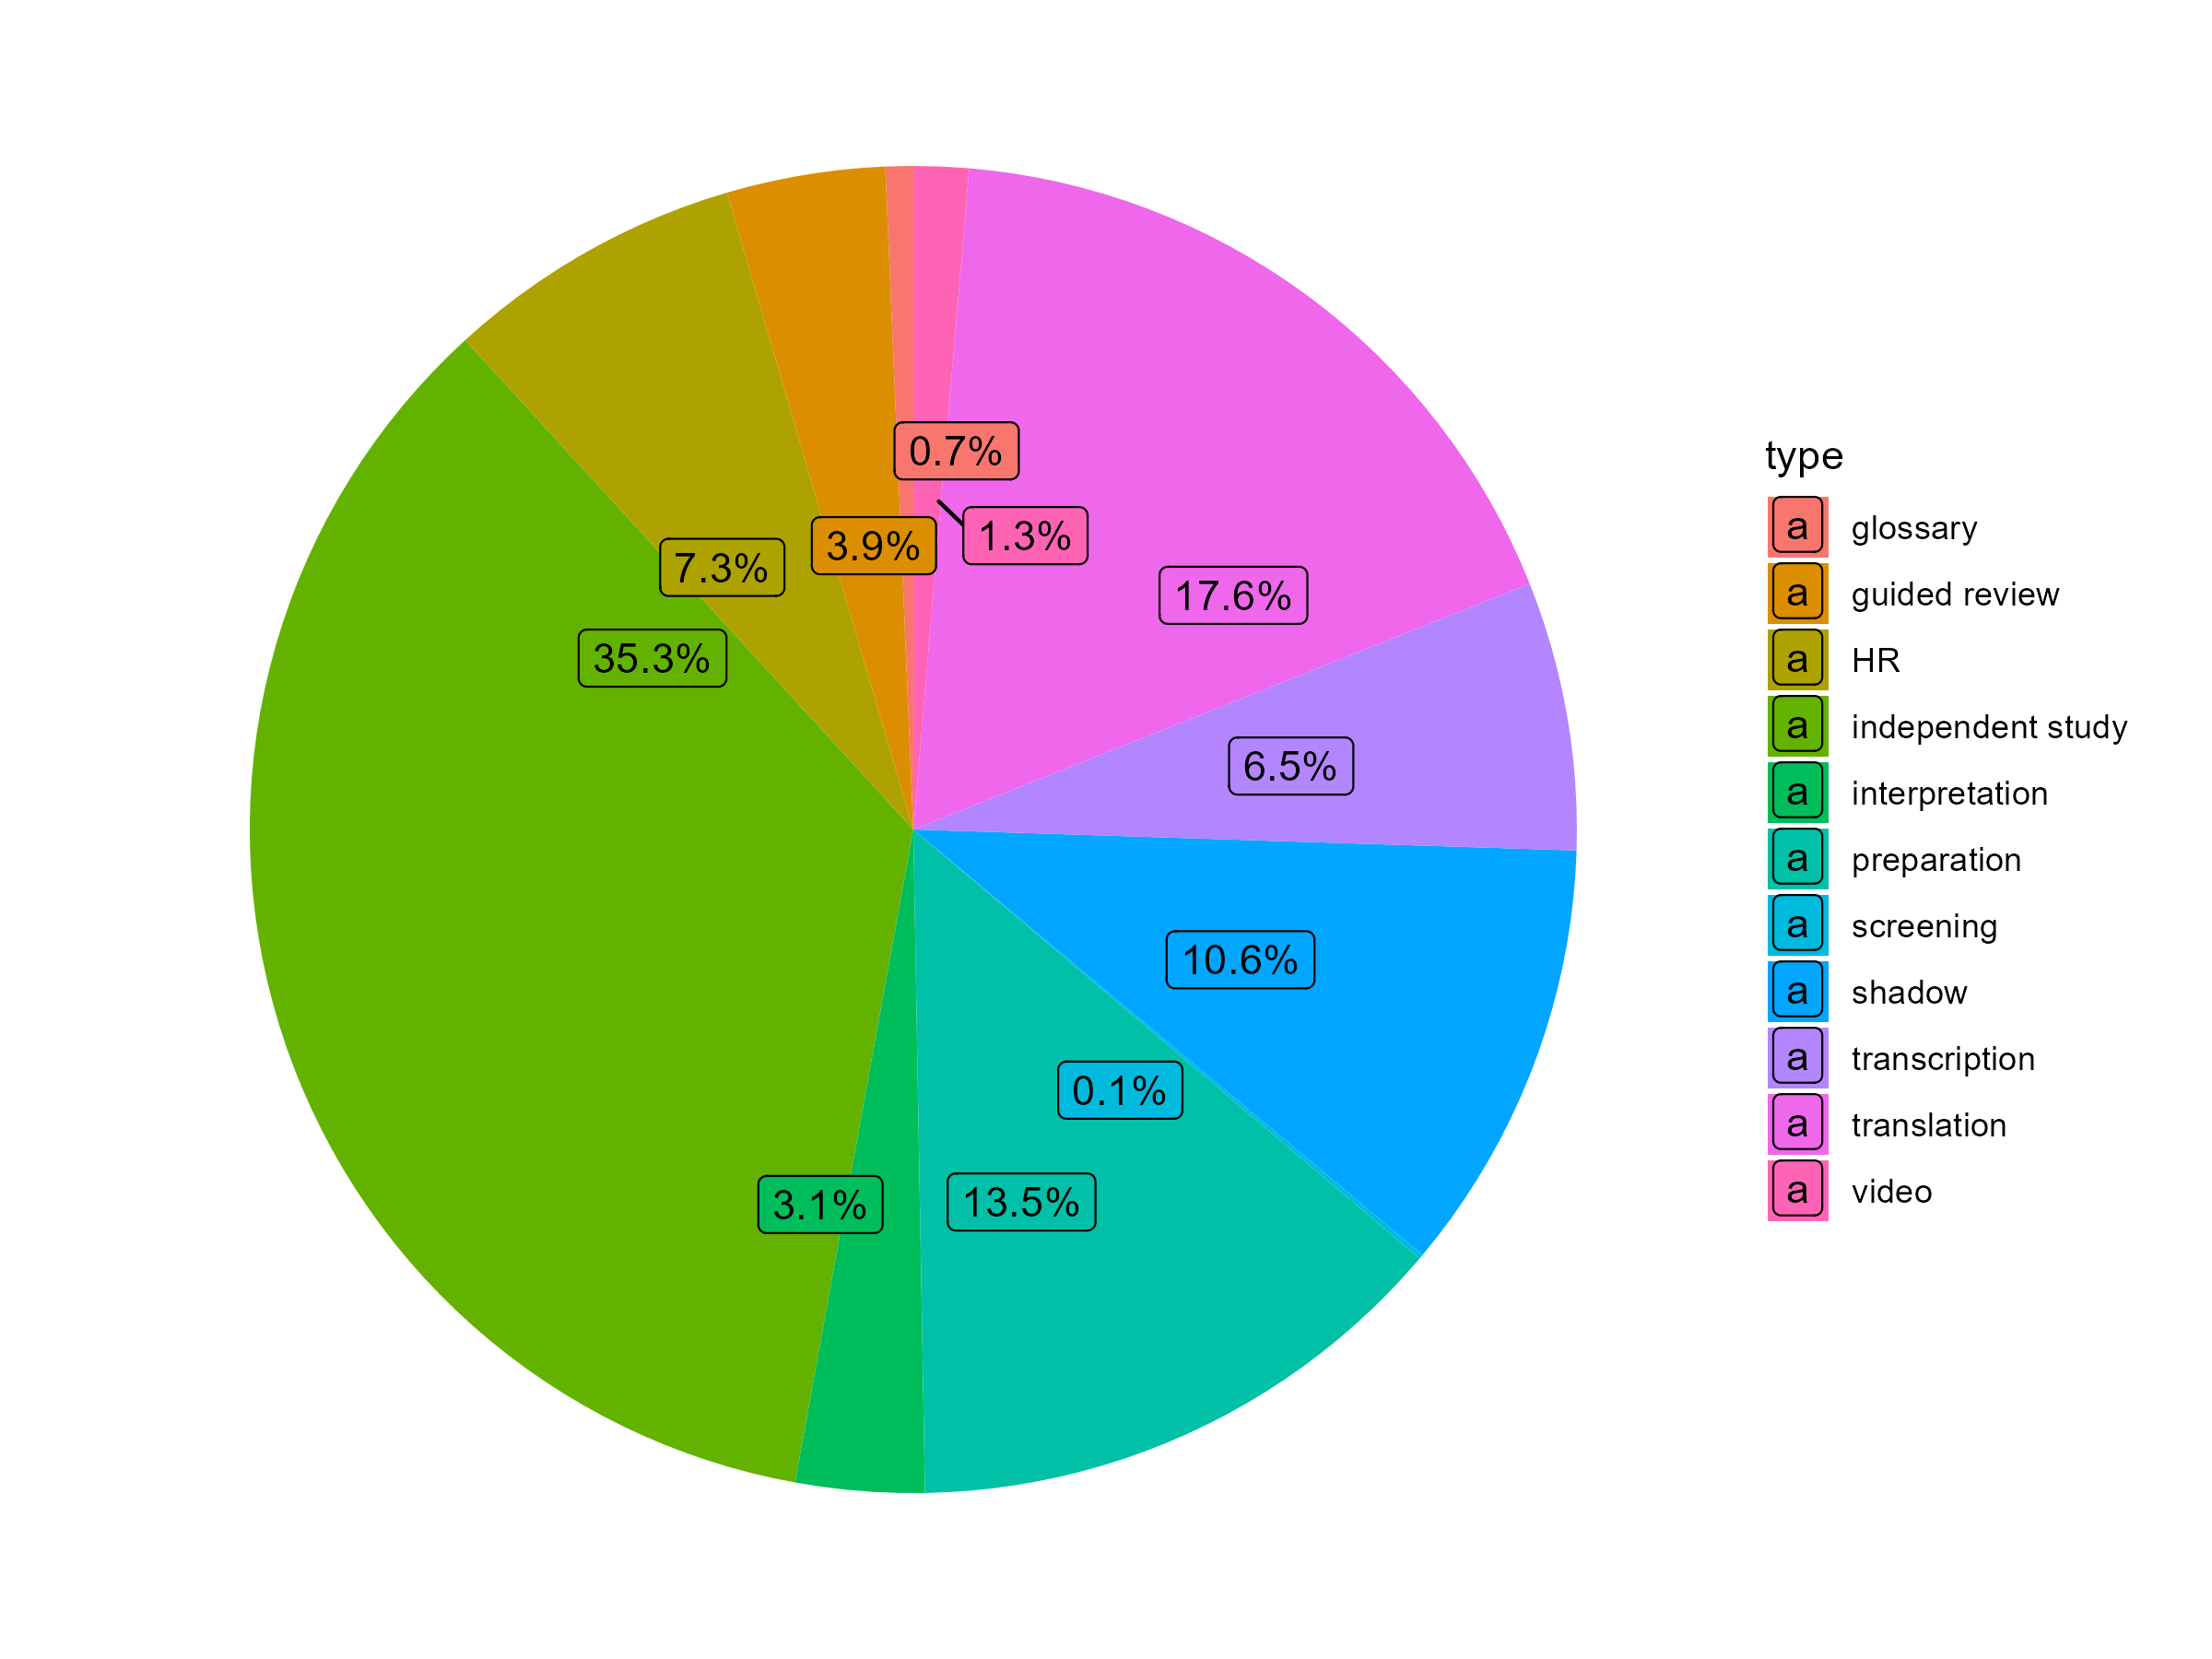
\includegraphics[width=\textwidth]{../figures/pie.png}
	\caption{Percentage of time spent on each task.}
	\label{fig:pie}
\end{figure}

\section{Conclusions}

Overall, I believe that the interpreting experiences that I had while at the Manhattan District Attorney’s Office have been extremely beneficial to me with long-lasting effects. At other interpreting jobs, I have been praised for my professionalism and effectiveness by service providers after encounters. The skills that I learned during my internship are what led to the professionalism that I was able to provide in those encounters.

The experience at the Manhattan District Attorney’s Office was unique and consequential to my development as an interpreter. Although I am not currently continuing to pursue a career in interpretation, I am still interested in maintaining my skills and eventually taking the New Jersey or New York court interpreting exam for freelancing purposes. This internship gave me greater insight into what would be expected of me, and what skills I need to continue working on if I would like to pursue this opportunity.

\appendix

\section{Sample Translation 1: Appeal}

The first document is an appeal for a verdict given in Puerto Rico. The typical challenges of legal translation were present in this document: the mismatch of two legal systems’ terminologies and complex syntax. For example, tribunal de primera instancia, which I found an equivalent in trial court. Another example is Transportación y Obras Públicas. Although the literal translation is straightforward (“Transportation and Public Works”), it is necessary to verify that this is the official or standard translation (which, it turns out, it is). This is especially pressing for a translation from Puerto Rico, for example, due to the bilingual nature of the country.

This text also demonstrates a mixture of high register and low register language. Although the majority of the text is produced by the court, which requires a high register with complex syntax, there is also a portion of the text handwritten by the appellant. This requires savviness on the translator’s part to accurately render the register differences into the target language. 

\subsection{Sample Translation 1: Appeal (source text)}

\begin{figure}[H]
	\centering
	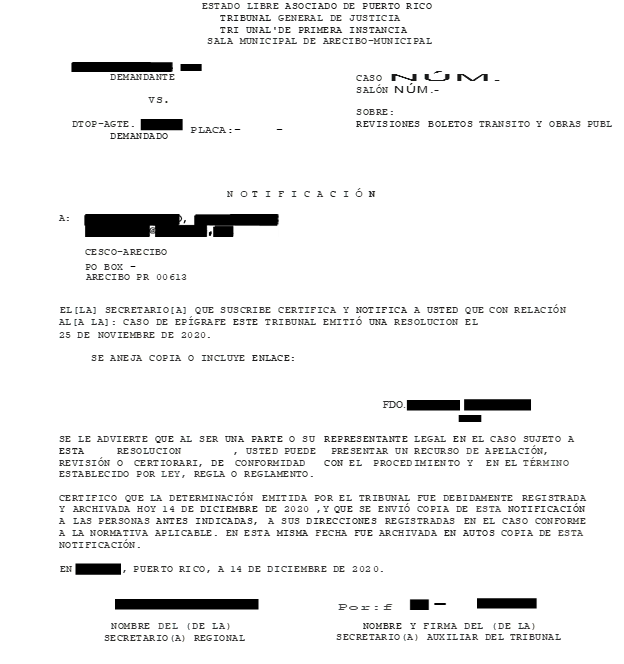
\includegraphics[width=\textwidth]{../sample_translations/source_1_1.png}
\end{figure}

\begin{figure}[H]
	\centering
	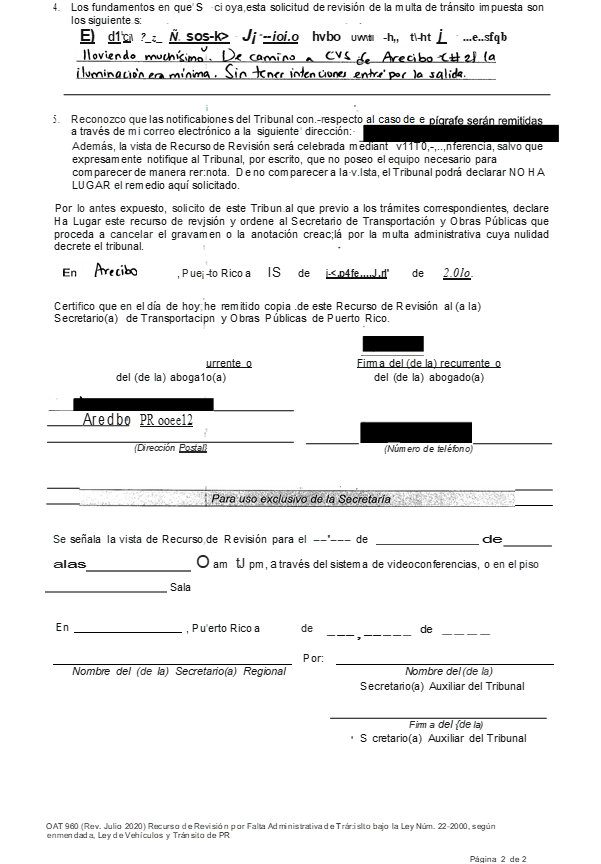
\includegraphics[width=\textwidth]{../sample_translations/source_1_2.png}
\end{figure}


\begin{figure}[H]
	\centering
	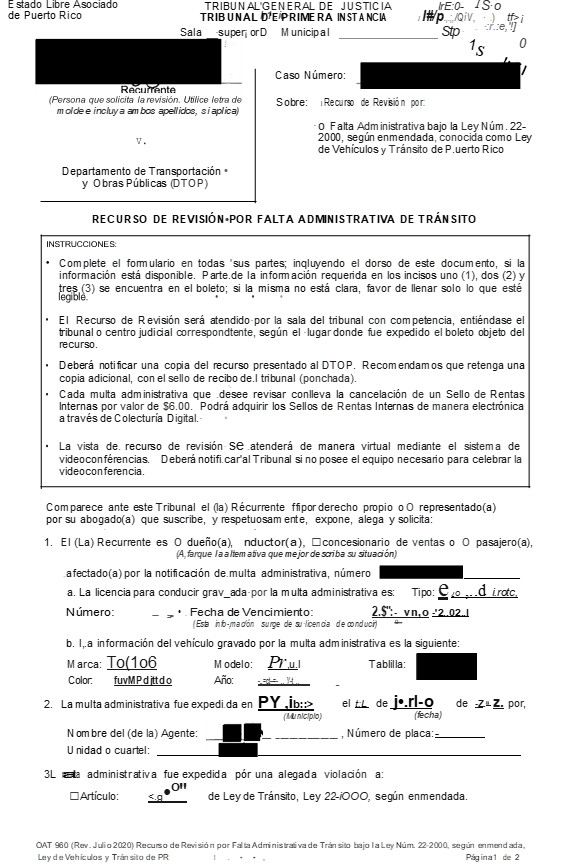
\includegraphics[width=\textwidth]{../sample_translations/source_1_3.png}
\end{figure}

\subsection{Sample Translation 1: Appeal (target text)}

\begin{figure}[H]
	\centering
	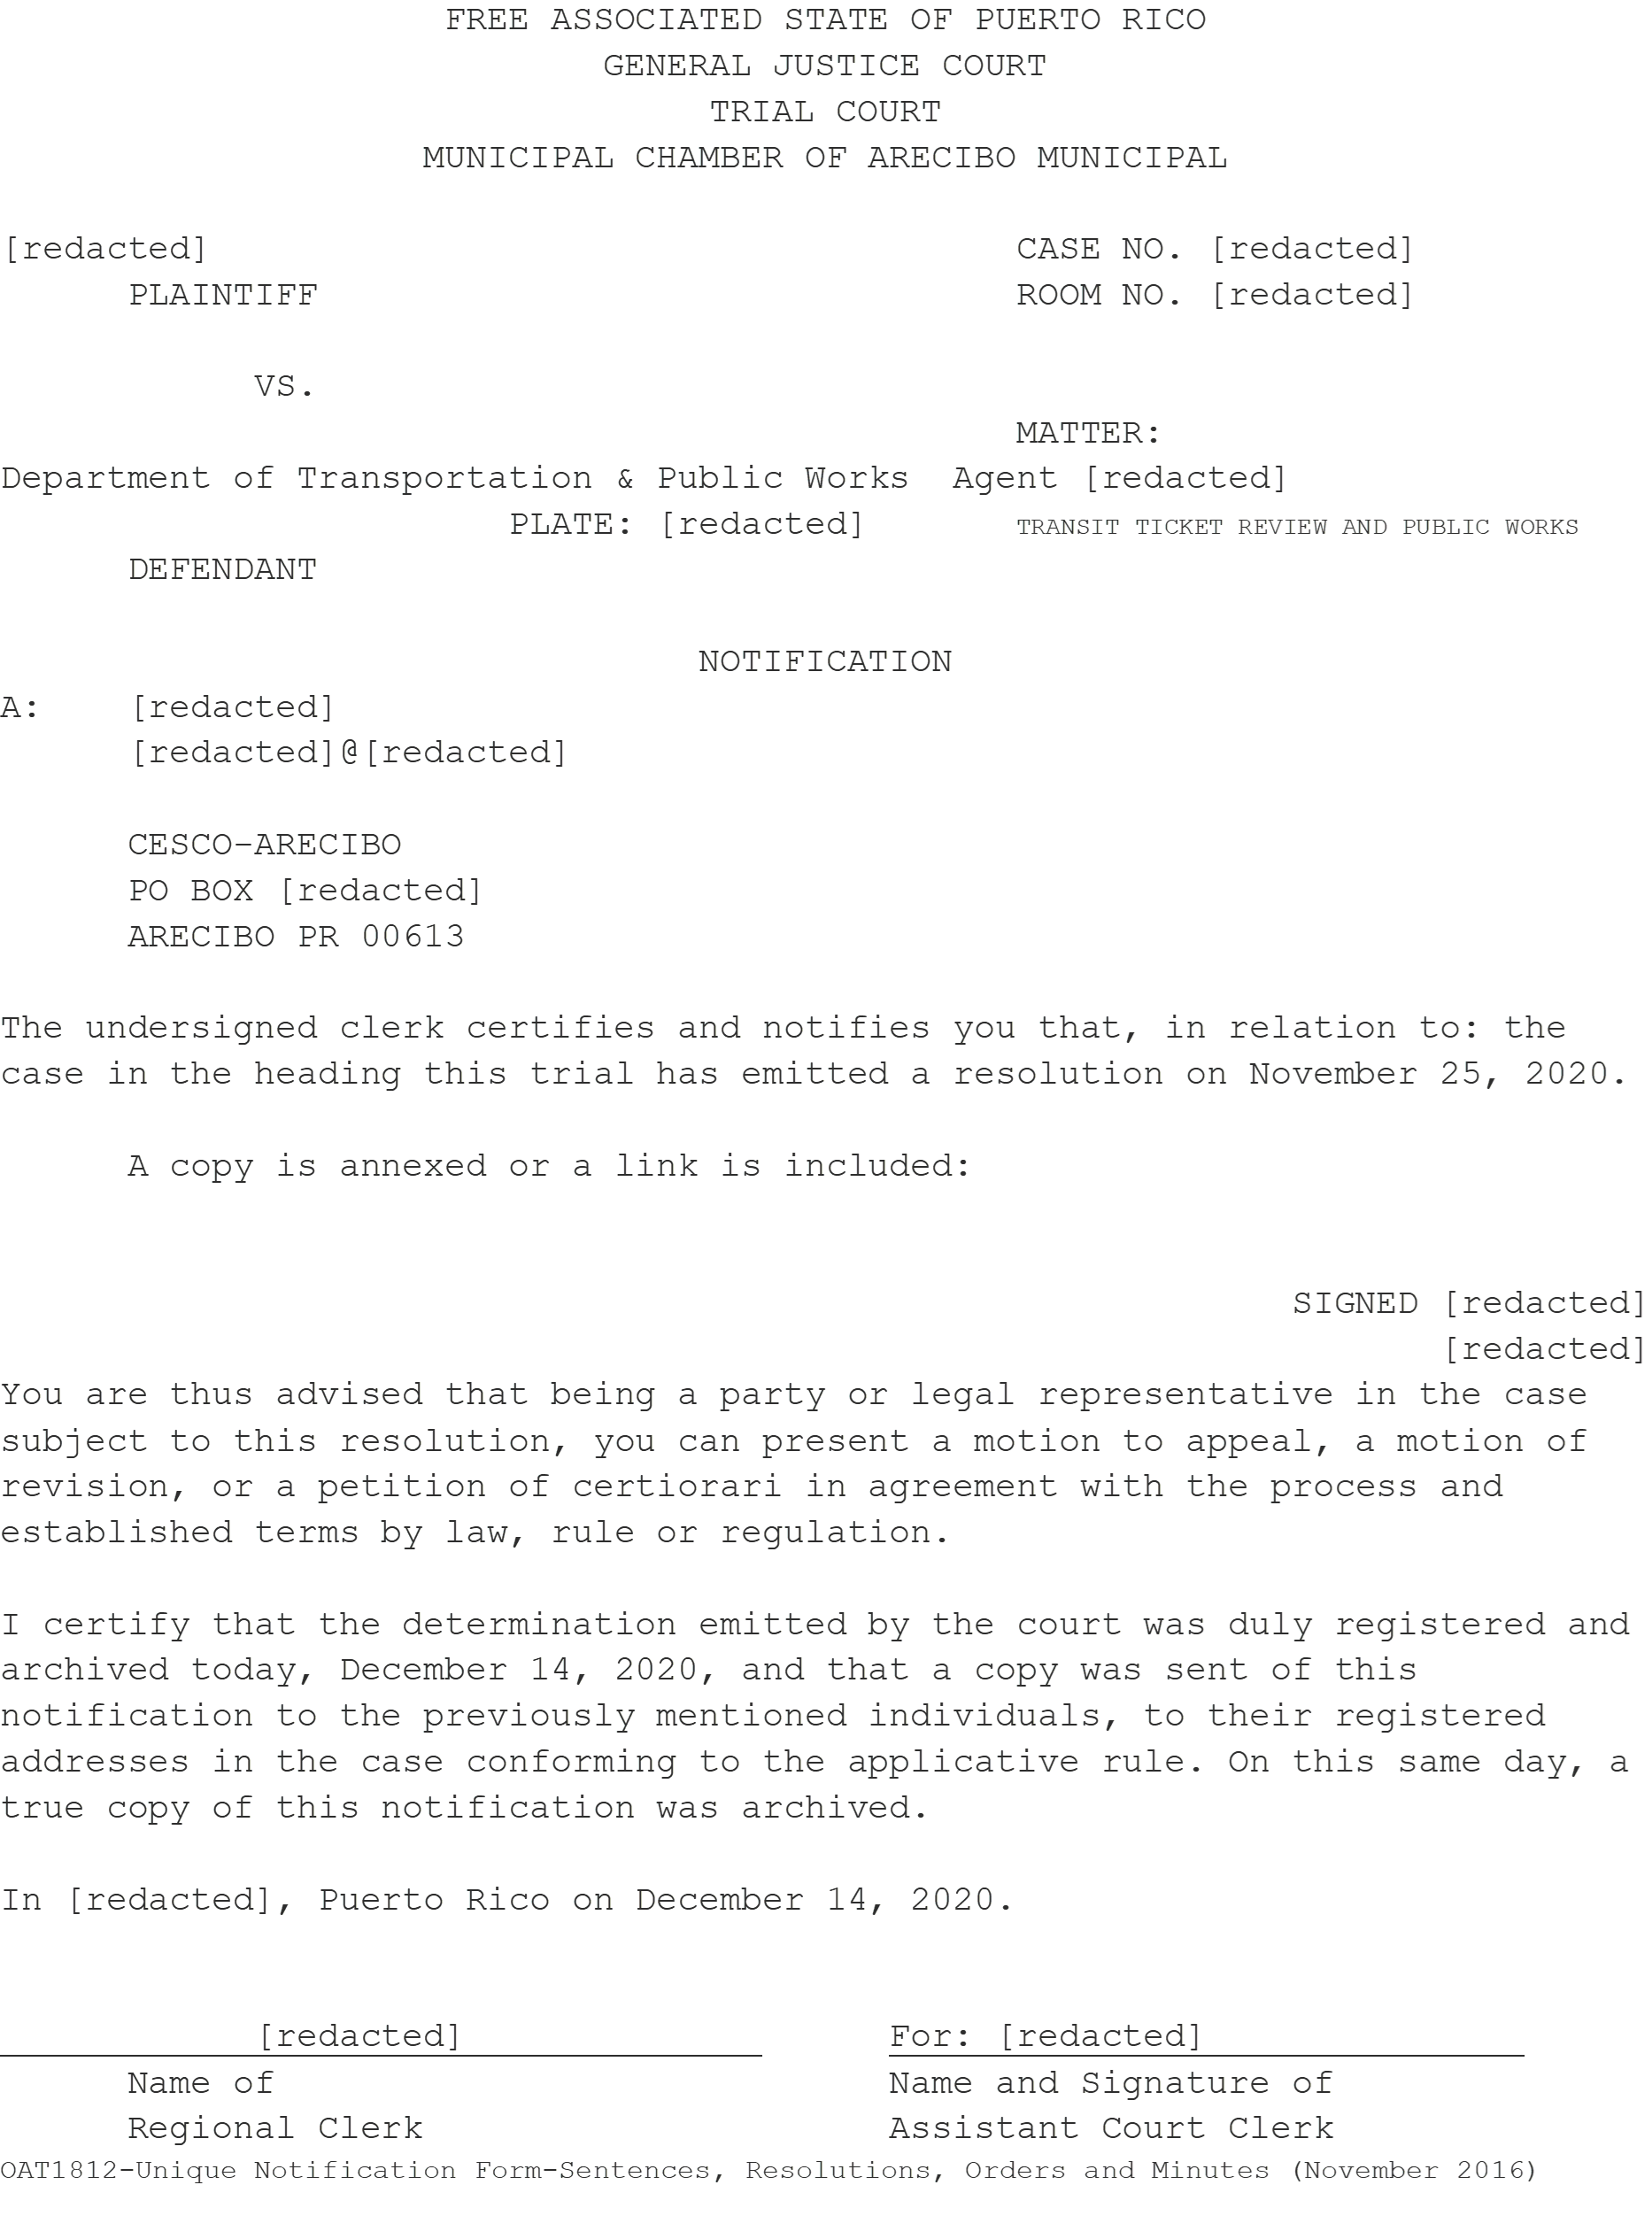
\includegraphics[width=\textwidth]{../sample_translations/target_1_1.png}
\end{figure}

\begin{figure}[H]
	\centering
	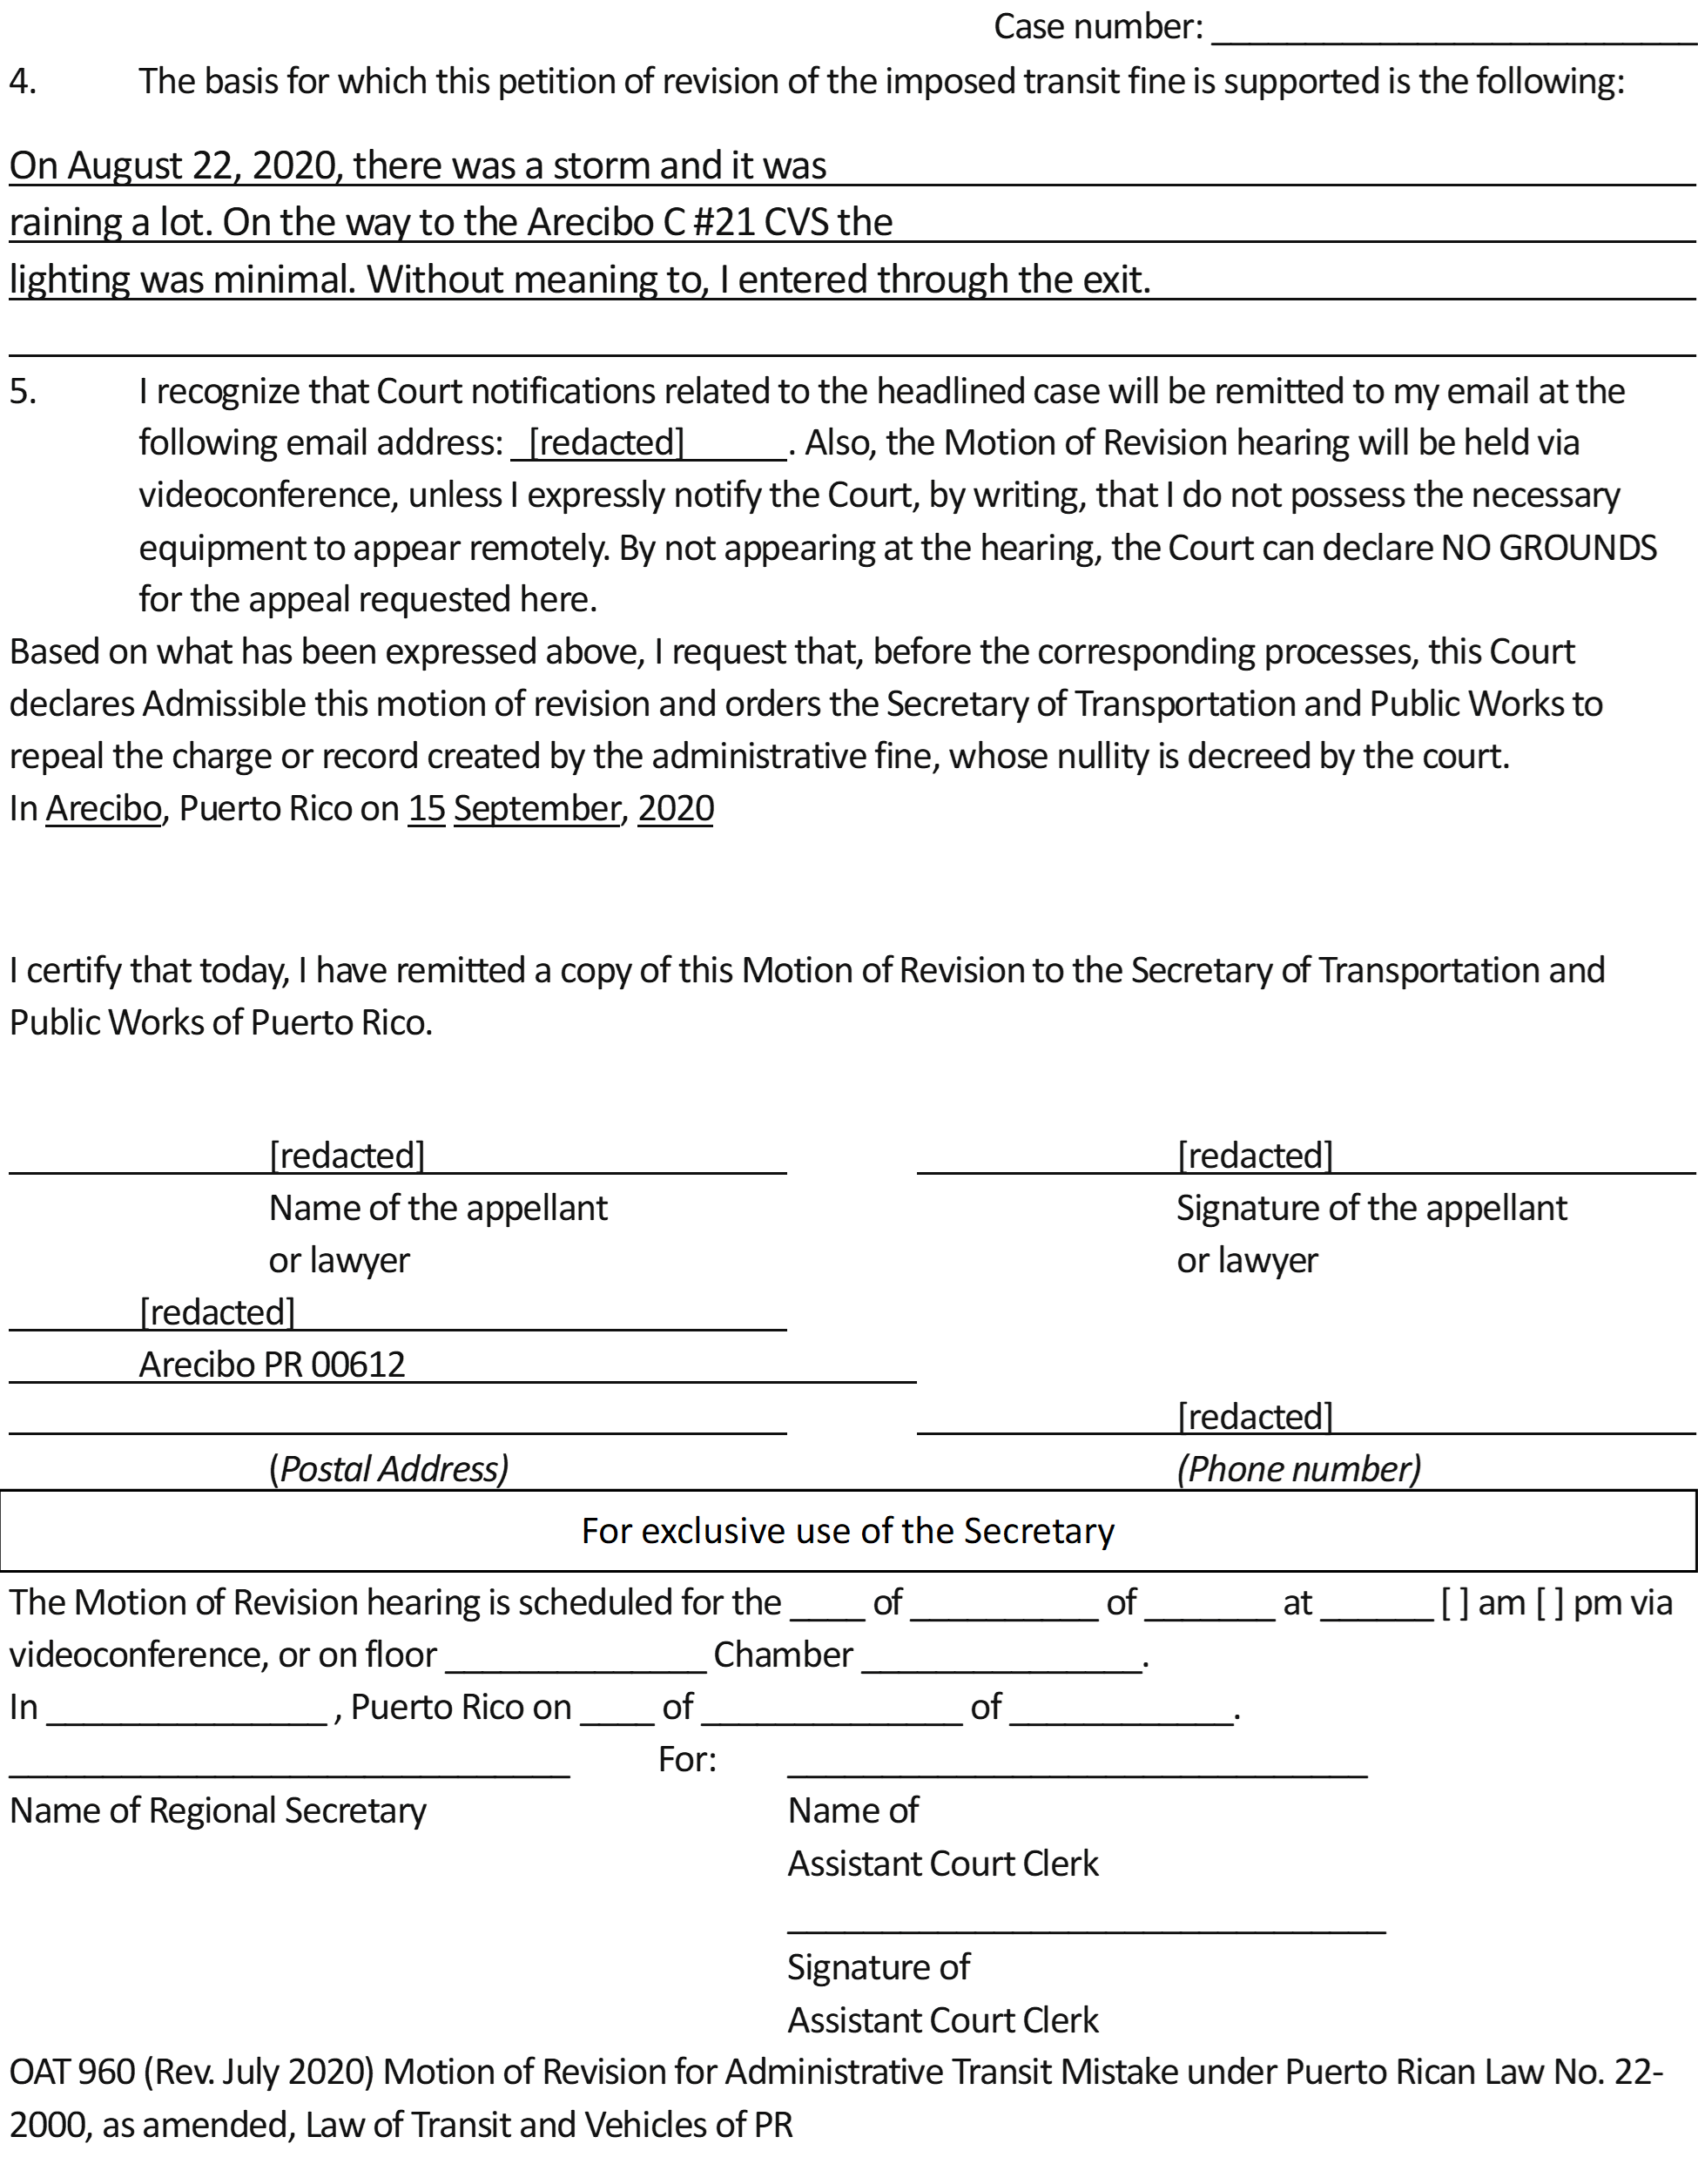
\includegraphics[width=\textwidth]{../sample_translations/target_1_2.png}
\end{figure}

\begin{figure}[H]
	\centering
	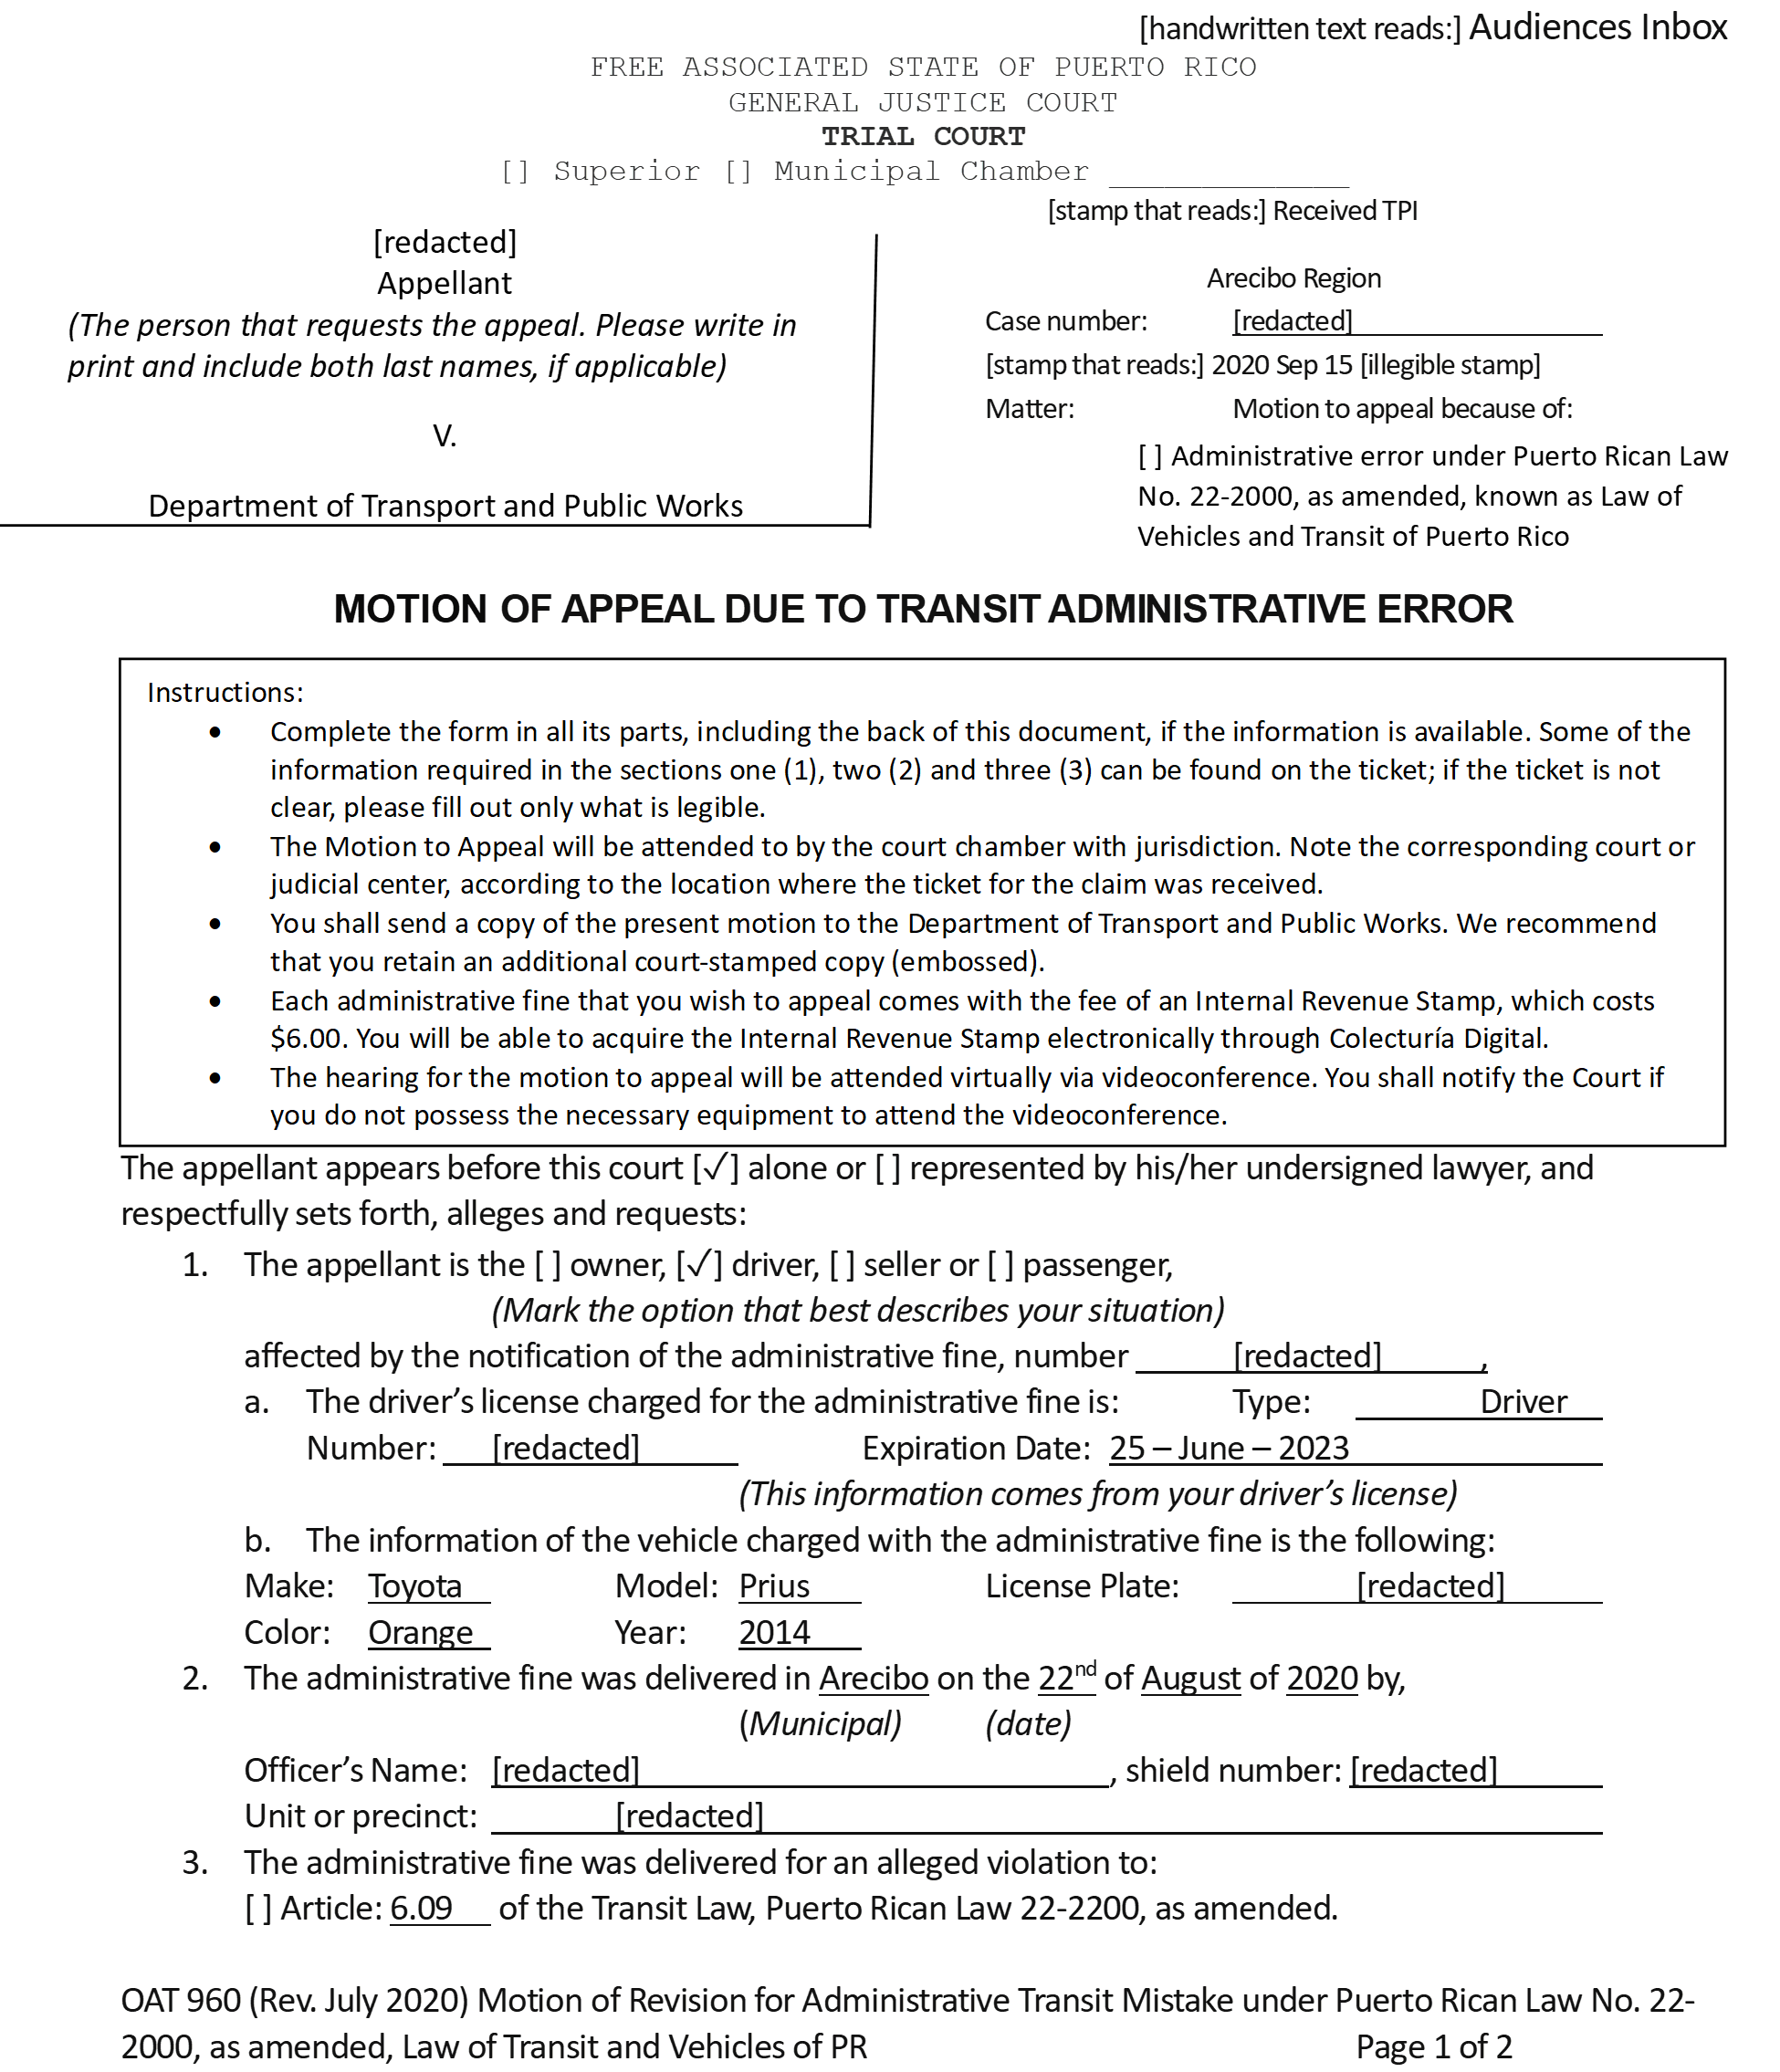
\includegraphics[width=\textwidth]{../sample_translations/target_1_3.png}
\end{figure}

\begin{figure}[H]
	\centering
	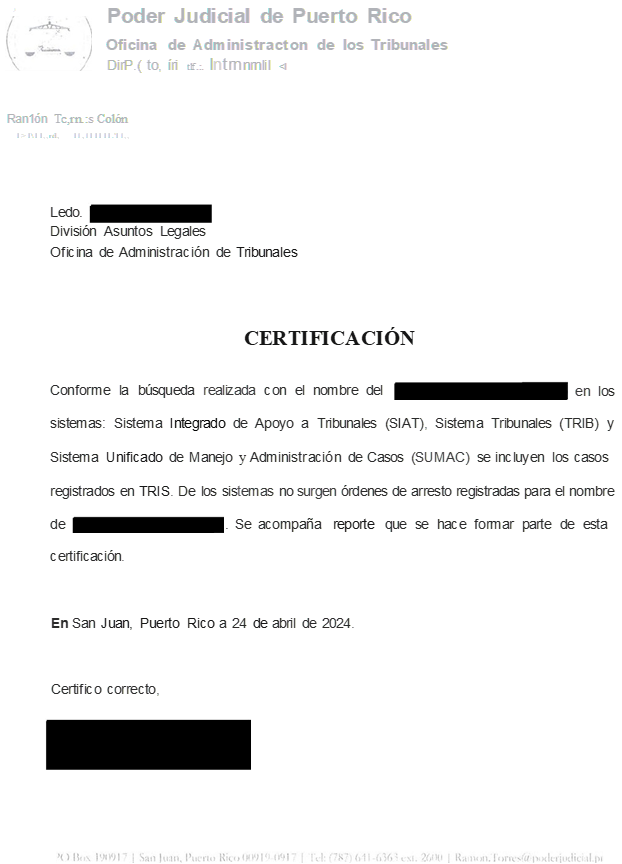
\includegraphics[width=\textwidth]{../sample_translations/target_1_4.png}
\end{figure}

SAMPLE

\section{Sample Translation 2: Subpoena Response}

The second text is a response to a subpoena, in this case, a demand to produce documents regarding the individual’s judicial history, from Puerto Rico. In this context, it is necessary to conform to the stylistic format of the target culture. Although Spanish legal texts tend to be verbose and syntactically complicated, this text did not present a major divergence from the equivalent text in English aimed at the American legal system.

\subsection{Sample Translation 2: Subpoena Response (source text)}

\begin{figure}[H]
	\centering
	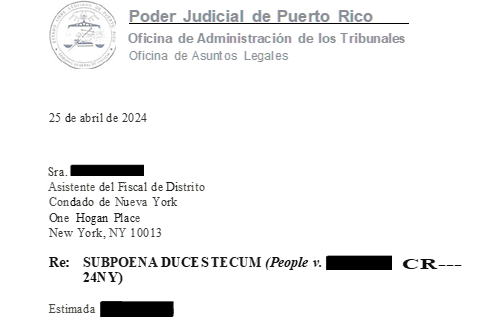
\includegraphics[width=\textwidth]{../sample_translations/source_2_1.png}
\end{figure}

\begin{figure}[H]
	\centering
	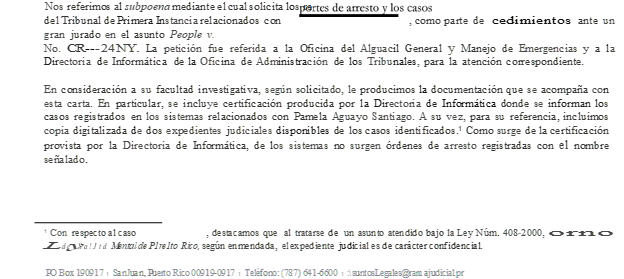
\includegraphics[width=\textwidth]{../sample_translations/source_2_2.png}
\end{figure}

\begin{figure}[H]
	\centering
	
\includegraphics[width=\textwidth]{../sample_translations/source_2_3.png}
\end{figure}

\subsection{Sample Translation 2: Subpoena Response (target text)}

\begin{figure}[H]
	\centering
	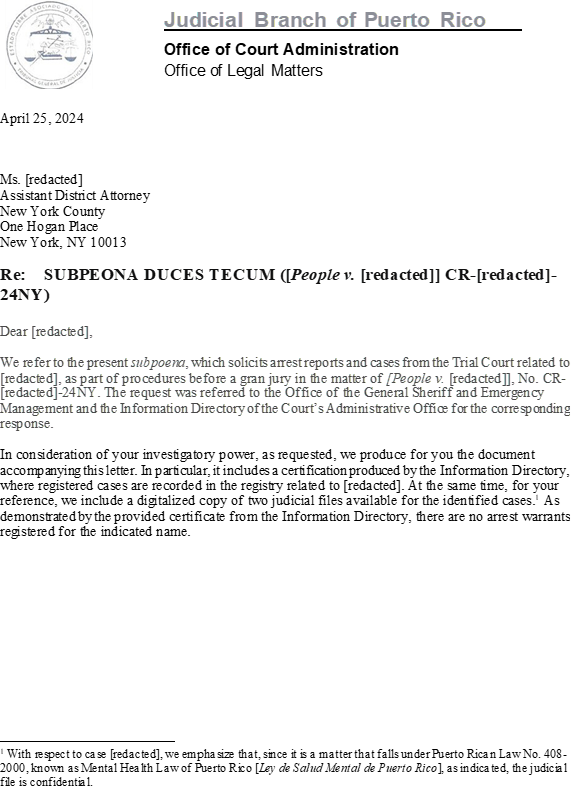
\includegraphics[width=\textwidth]{../sample_translations/target_2_1.png}
\end{figure}

\begin{figure}[H]
	\centering
	
\includegraphics[width=\textwidth]{../sample_translations/target_2_2.png}
\end{figure}

\begin{figure}[H]
	\centering
	
\includegraphics[width=\textwidth]{../sample_translations/target_2_3.png}
\end{figure}
\newpage

\bibliography{references}
\

\end{document}